
% Spatial Adaptive FSP — talk
% Aditya Dendukuri

\documentclass[10pt,aspectratio=169]{beamer}

\usetheme{Boadilla}
\usecolortheme{seahorse}
\setbeamertemplate{navigation symbols}{}
\setbeamerfont{frametitle}{size=\normalsize,series=\bfseries}
\setbeamerfont{title}{size=\large,series=\bfseries}

\usepackage{amsmath,amssymb,bm,mathtools}
\usepackage{tikz}
\usetikzlibrary{arrows.meta,positioning,patterns,decorations.pathreplacing,calc,shapes.geometric}
\usepackage{graphicx}
\usepackage{booktabs}
\usepackage{xcolor}

\graphicspath{{figures/}{../examples/output/}}

\newcommand{\Pois}{\operatorname{Pois}}
\newcommand{\Bin}{\operatorname{Bin}}
\newcommand{\calR}{\mathcal{R}}
\newcommand{\calP}{\mathcal{P}}
\newcommand{\citeref}[1]{{\scriptsize\textcolor{gray}{[#1]}}}

\definecolor{fastblue}{RGB}{31,119,180}
\definecolor{slowred}{RGB}{214,39,40}
\definecolor{myblue}{RGB}{31,119,180}
\definecolor{mygray}{RGB}{80,80,80}
\definecolor{activecolor}{RGB}{220,100,20}    % orange — active voxels
\definecolor{equilcolor}{RGB}{70,130,200}     % steel blue — equilibrated
\definecolor{emptycolor}{RGB}{50,50,50}       % dark — empty
\definecolor{coarsegreen}{RGB}{44,160,44}

\title[Spatial Adaptive FSP]{%
  A Spatially Adaptive Finite State Projection\\
  for the Reaction-Diffusion Master Equation}
\author{Aditya Dendukuri}
\institute[UCSB]{University of California, Santa Barbara}
\date{}

\begin{document}

\begin{frame}\titlepage\end{frame}


% ================================================================
% 1. CME
% ================================================================
\begin{frame}{The Chemical Master Equation (CME)}

  \begin{columns}[T]
    \begin{column}{0.52\textwidth}
      A \textbf{single well-mixed compartment} holding molecules of $S$ species.
      State: molecule count vector $\bm{n} \in \mathbb{Z}_{\ge 0}^S$.

      \medskip
      Each reaction $r$ fires with rate $\alpha_r(\bm{n})$ and changes the state
      by stoichiometry $\bm{\nu}_r$.
      The probability distribution $p(\bm{n},t)$ evolves as

      \[
        \frac{dp}{dt} = \underbrace{Ap}_{\text{CME}},
      \]
      where $A_{ij} = \alpha_r(\bm{n}_j)$ if $\bm{n}_i = \bm{n}_j + \bm{\nu}_r$,
      and the diagonal ensures column sums are zero.

      \bigskip
      \begin{block}{Finite State Projection (FSP)}
        Truncate to a finite support $\mathcal{S}$; expand it adaptively as
        probability mass spreads.  State space $|\mathcal{S}|$ grows only as
        needed --- not exponentially in time.
      \end{block}
    \end{column}
    \begin{column}{0.44\textwidth}
      \begin{center}
      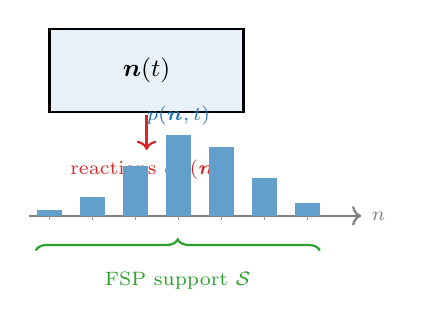
\begin{tikzpicture}[scale=0.88, every node/.style={font=\small}]
        % single voxel box
        \draw[thick,fill=myblue!10] (0,0) rectangle (2.8,1.2);
        \node at (1.4,0.6) {$\bm{n}(t)$};
        \draw[->,slowred,thick] (1.4,-0.05) -- (1.4,-0.55)
          node[below,font=\scriptsize]{reactions $\alpha_r(\bm{n})$};

        % 1-D state space below
        \draw[->,black!50,thick] (-0.3,-1.5) -- (4.5,-1.5)
          node[right,font=\scriptsize]{$n$};
        \foreach \n in {0,1,2,3,4,5,6}
          \draw[black!40,thin] (\n*0.62,-1.56) -- (\n*0.62,-1.44);
        \foreach \n/\h in {0/0.05, 1/0.15, 2/0.40, 3/0.65, 4/0.55, 5/0.30, 6/0.10}
          \fill[myblue!70] (\n*0.62-0.18,-1.5) rectangle (\n*0.62+0.18,-1.5+\h*1.8);
        \node[above,myblue,font=\scriptsize] at (1.86,-1.5+0.65*1.8) {$p(\bm{n},t)$};

        % FSP bracket
        \draw[decorate,decoration={brace,amplitude=4pt},thick,coarsegreen]
          (-0.2,-2.0) -- (3.72+0.18,-2.0)
          node[midway,below=4pt,font=\scriptsize,coarsegreen]{FSP support $\mathcal{S}$};
      \end{tikzpicture}
      \end{center}
    \end{column}
  \end{columns}

\end{frame}


% ================================================================
% 2. RDME: K coupled CMEs
% ================================================================
\begin{frame}{The RDME: $K$ coupled CMEs}

  \begin{columns}[T]
    \begin{column}{0.50\textwidth}
      Divide the spatial domain into $K$ voxels of width $h$.
      Each voxel $k$ has its own count vector $\bm{n}_k$ and \textbf{its own CME}.

      \medskip
      Voxels are coupled by \textbf{diffusion}: one molecule hops $k\leftrightarrow k{\pm}1$
      at rate $d = D/h^2$ per molecule.

      \medskip
      The joint distribution $p(\bm{n}_1,\ldots,\bm{n}_K,t)$ obeys

      \[
        \frac{dp}{dt} = \underbrace{(A_{\rm rxn} + A_{\rm diff})}_{\displaystyle A_{\rm RDME}}\,p.
      \]

      \vspace{0.3em}
      \begin{alertblock}{Exponential cost}
        Full state space: $n_{\max}^{SK}$.\\
        Even $K{=}8$, $S{=}1$, $n_{\max}{=}50$: intractable.\\[0.2em]
        $A_{\rm RDME}$ is \textbf{block-tridiagonal}: $A_k$ on diagonal (CME),
        $D_{k,k+1}$ off-diagonal (diffusion shifts one count).
      \end{alertblock}
    \end{column}
    \begin{column}{0.46\textwidth}
      \begin{center}
      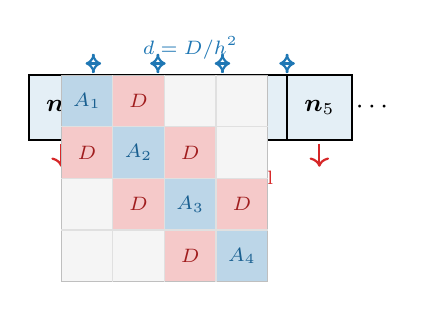
\begin{tikzpicture}[scale=0.82, every node/.style={font=\small}]
        \foreach \k in {1,2,3,4,5} {
          \draw[thick,fill=myblue!12] (\k-1,0) rectangle (\k,1.0);
          \node at (\k-0.5, 0.50) {$\bm{n}_\k$};
        }
        \node[font=\normalsize] at (5.35,0.5) {$\cdots$};
        \foreach \k in {1,2,3,4} {
          \draw[<->,fastblue,thick] (\k-0.12,1.18) -- (\k+0.12,1.18);
        }
        \node[fastblue,font=\scriptsize] at (2.5,1.42) {$d = D/h^2$};
        \foreach \k in {1,2,3,4,5} {
          \draw[->,slowred,thick] (\k-0.5,-0.06) -- (\k-0.5,-0.42);
        }
        \node[slowred,font=\scriptsize] at (2.5,-0.62) {$\alpha_r(\bm{n}_k)$ per voxel};

        % block-tridiagonal schematic
        \def\bs{0.80}
        \begin{scope}[yshift=-2.2cm, xshift=0.5cm]
          \fill[gray!8] (0,0) rectangle (4*\bs,4*\bs);
          \foreach \k in {0,1,2,3}
            \fill[myblue!30] (\k*\bs,{(3-\k)*\bs}) rectangle
                             ({(\k+1)*\bs},{(4-\k)*\bs});
          \foreach \k in {0,1,2} {
            \fill[slowred!25] ({(\k+1)*\bs},{(3-\k)*\bs}) rectangle
                              ({(\k+2)*\bs},{(4-\k)*\bs});
            \fill[slowred!25] ({\k*\bs},{(2-\k)*\bs}) rectangle
                              ({(\k+1)*\bs},{(3-\k)*\bs});
          }
          \draw[black!25] (0,0) rectangle (4*\bs,4*\bs);
          \foreach \k in {1,2,3} {
            \draw[black!12,thin] (\k*\bs,0)--(\k*\bs,4*\bs);
            \draw[black!12,thin] (0,\k*\bs)--(4*\bs,\k*\bs);
          }
          \foreach \k/\l in {0/$A_1$,1/$A_2$,2/$A_3$,3/$A_4$}
            \node[font=\scriptsize,myblue!80!black]
              at ({(\k+0.5)*\bs},{(3.5-\k)*\bs}) {\l};
          \foreach \k/\l in {0/$D$,1/$D$,2/$D$} {
            \node[font=\scriptsize,slowred!75!black]
              at ({(\k+1.5)*\bs},{(3.5-\k)*\bs}) {\l};
            \node[font=\scriptsize,slowred!75!black]
              at ({(\k+0.5)*\bs},{(2.5-\k)*\bs}) {\l};
          }
        \end{scope}
      \end{tikzpicture}
      \end{center}
    \end{column}
  \end{columns}

\end{frame}


% ================================================================
% 3. Key observation: spatial sparsity
% ================================================================
\begin{frame}{Key observation: molecules don't teleport}

  \begin{columns}[T]
    \begin{column}{0.50\textwidth}
      Starting from a \textbf{localised initial condition} (all molecules in one
      region), probability mass spreads \emph{diffusively}.

      \medskip
      At any time $t$, the support of $p$ is concentrated near the
      \textbf{diffusion wavefront}: voxels far from the origin are essentially empty.

      \bigskip
      \textbf{Three regimes} at any instant:
      \medskip
      \begin{itemize}\setlength\itemsep{0.5em}
        \item[\textcolor{emptycolor}{\rule{8pt}{8pt}}]
              \textbf{Empty}: $p(\bm{n}_k) \approx \delta_{\bm{n}_k,\bm{0}}$.
              No tracking needed.
        \item[\textcolor{activecolor}{\rule{8pt}{8pt}}]
              \textbf{Active}: wavefront voxels. Nontrivial distribution —
              track with the full CME.
        \item[\textcolor{equilcolor}{\rule{8pt}{8pt}}]
              \textbf{Equilibrated}: behind the wavefront, distribution
              has converged to a known form. Store as a single parameter.
      \end{itemize}
    \end{column}
    \begin{column}{0.46\textwidth}
      \begin{center}
      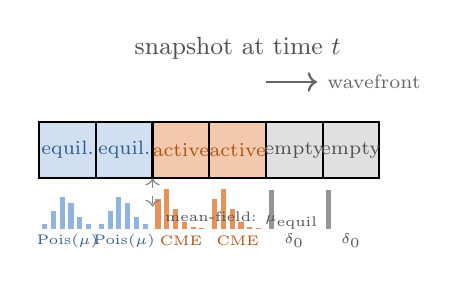
\begin{tikzpicture}[scale=0.72]
        \def\K{6}
        % time label
        \node[font=\small,mygray] at (3.5,4.8) {snapshot at time $t$};

        % row of voxels
        \foreach \k in {1,...,\K} {
          \pgfmathtruncatemacro{\state}{
            (\k<=2) ? 2 : ((\k==3 || \k==4) ? 1 : 0)
          }
          \ifnum\state=2
            \draw[thick,fill=equilcolor!25] (\k-1,2.5) rectangle (\k,3.5);
          \fi
          \ifnum\state=1
            \draw[thick,fill=activecolor!35] (\k-1,2.5) rectangle (\k,3.5);
          \fi
          \ifnum\state=0
            \draw[thick,fill=emptycolor!15] (\k-1,2.5) rectangle (\k,3.5);
          \fi
        }
        % voxel labels
        \node[font=\scriptsize,equilcolor!70!black] at (0.5,3.0)  {equil.};
        \node[font=\scriptsize,equilcolor!70!black] at (1.5,3.0)  {equil.};
        \node[font=\scriptsize,activecolor!80!black] at (2.5,3.0) {active};
        \node[font=\scriptsize,activecolor!80!black] at (3.5,3.0) {active};
        \node[font=\scriptsize,mygray]              at (4.5,3.0)  {empty};
        \node[font=\scriptsize,mygray]              at (5.5,3.0)  {empty};

        % wavefront arrow
        \draw[->,thick,black!60] (4.0,4.2) -- (4.9,4.2)
          node[right,font=\scriptsize]{wavefront};

        % distribution sketches below each voxel
        % equil: Poisson bars
        \foreach \k in {1,2} {
          \foreach \n/\h in {0/0.05,1/0.18,2/0.32,3/0.26,4/0.12,5/0.05} {
            \fill[equilcolor!60]
              ({\k-1+\n*0.155+0.05},1.6) rectangle
              ({\k-1+\n*0.155+0.14},1.6+\h*1.8);
          }
          \node[equilcolor!70!black,font=\tiny] at (\k-0.5,1.4) {$\Pois(\mu)$};
        }
        % active: broader/asymmetric bars
        \foreach \k in {3,4} {
          \foreach \n/\h in {0/0.30,1/0.40,2/0.20,3/0.07,4/0.02,5/0.01} {
            \fill[activecolor!70]
              ({\k-1+\n*0.155+0.05},1.6) rectangle
              ({\k-1+\n*0.155+0.14},1.6+\h*1.8);
          }
          \node[activecolor!80!black,font=\tiny] at (\k-0.5,1.4) {CME};
        }
        % empty: spike at 0
        \foreach \k in {5,6} {
          \fill[mygray!60] ({\k-1+0.05},1.6) rectangle ({\k-1+0.14},1.6+0.7);
          \node[mygray,font=\tiny] at (\k-0.5,1.4) {$\delta_0$};
        }

        % mean-field coupling annotation
        \draw[<->,dashed,black!50,thin] (2.0,2.5) -- (2.0,2.0);
        \node[font=\tiny,mygray,right] at (2.05,1.75) {mean-field: $\mu_{\rm equil}$};
      \end{tikzpicture}
      \end{center}
    \end{column}
  \end{columns}

\end{frame}


% ================================================================
% 4. Mean-field coupling
% ================================================================
\begin{frame}{Mean-field coupling: exact for linear kinetics}

  \begin{columns}[T]
    \begin{column}{0.52\textwidth}
      \textbf{Exact RDME:} gain rate into voxel $k$ from neighbor $\ell$ is
      $d \cdot n_\ell$, which depends on the \emph{random} count $n_\ell$.

      \medskip
      \textbf{Mean-field approximation:} replace the random $n_\ell$ by its mean
      $\mu_\ell = \mathbb{E}[n_\ell]$, decoupling the voxel CMEs:

      \[
        \frac{d p_k}{dt} = Q_k(\mu_{\rm nbr})\,p_k,
      \]
      where the effective generator has
      \[
        k_b^{\rm eff} = k_b + d\!\sum_{\ell \sim k} \mu_\ell, \qquad
        k_d^{\rm eff} = k_d + d\,|\text{nbrs}|.
      \]

      \medskip
      \begin{block}{When is mean-field exact?}
        For \textbf{linear (birth-death) kinetics}, the SS is a product of
        independent Poissons: $p^* = \prod_k \Pois(\mu^*)$.
        Detailed balance holds under symmetric diffusion, so mean-field is
        \textbf{exact at steady state}.
        \citeref{Isaacson 2009}
      \end{block}
    \end{column}
    \begin{column}{0.44\textwidth}
      \begin{center}
      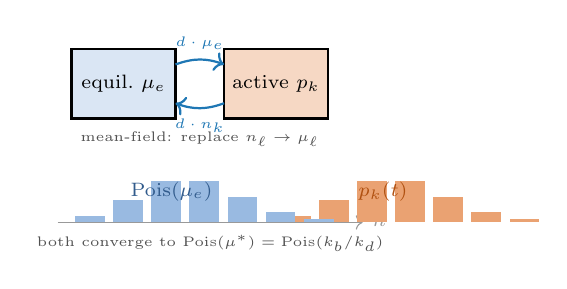
\begin{tikzpicture}[scale=0.88, every node/.style={font=\scriptsize}]
        % Two-voxel detailed balance
        \draw[thick,fill=equilcolor!20] (0,2.0) rectangle (1.5,3.0);
        \draw[thick,fill=activecolor!25] (2.2,2.0) rectangle (3.7,3.0);
        \node at (0.75,2.5) {equil.~$\mu_e$};
        \node at (2.95,2.5) {active $p_k$};

        \draw[->,fastblue,thick,bend left=20] (1.5,2.78) to
          node[above,font=\tiny]{$d\cdot\mu_e$} (2.2,2.78);
        \draw[->,fastblue,thick,bend left=20] (2.2,2.22) to
          node[below,font=\tiny]{$d\cdot n_k$} (1.5,2.22);

        \node[mygray,font=\tiny] at (1.85,1.7)
          {mean-field: replace $n_\ell \to \mu_\ell$};

        % Local SS diagram
        \draw[->,black!40,thin] (-0.2,0.5) -- (4.2,0.5) node[right]{$n$};
        \foreach \n/\h in {0/0.04,1/0.15,2/0.27,3/0.27,4/0.17,5/0.07,6/0.02} {
          \fill[equilcolor!55] ({\n*0.55+0.05},0.5) rectangle
            ({\n*0.55+0.48},0.5+\h*2.2);
          \fill[activecolor!60] ({\n*0.55+3.02},0.5) rectangle
            ({\n*0.55+3.45},0.5+\h*2.2);
        }
        \node[equilcolor!70!black] at (0.75*0.55*3.5,0.95) {$\Pois(\mu_e)$};
        \node[activecolor!80!black] at (3.05+0.75*0.55*3.5,0.95) {$p_k(t)$};
        \node[mygray,font=\tiny] at (2.0,0.2)
          {both converge to $\Pois(\mu^*) = \Pois(k_b/k_d)$};
      \end{tikzpicture}
      \end{center}
    \end{column}
  \end{columns}

\end{frame}


% ================================================================
% 5. The adaptive cycle
% ================================================================
\begin{frame}{The adaptive FSP cycle: Prolong $\to$ Evolve $\to$ Restrict}

\vspace{-0.2cm}
\begin{center}
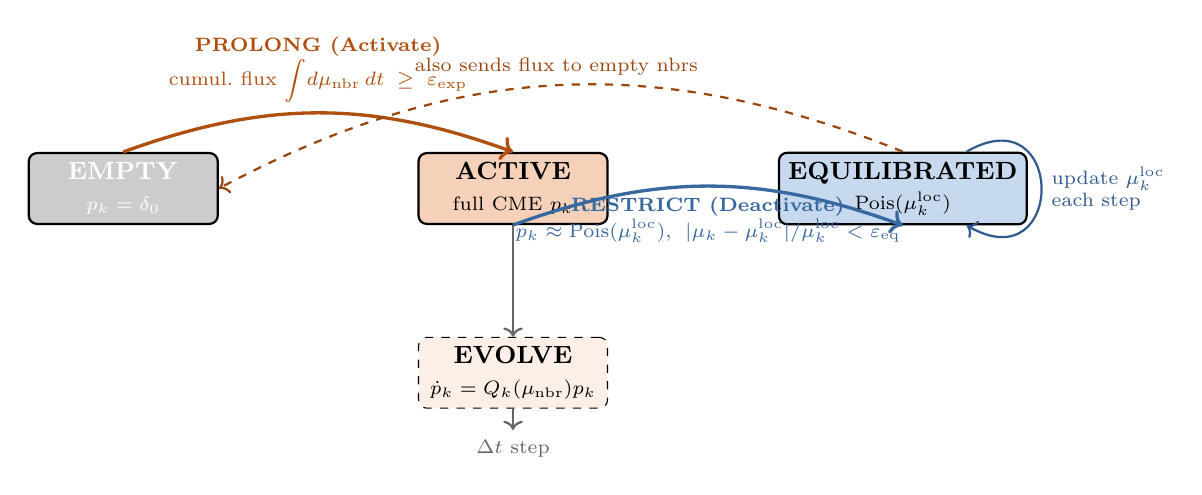
\begin{tikzpicture}[scale=0.90, every node/.style={font=\small},
    box/.style={draw,rounded corners=3pt,minimum width=2.4cm,
                minimum height=0.9cm,align=center,thick}]

  % Three state boxes (top)
  \node[box,fill=emptycolor!25,text=white]      (empty) at (0,0)
    {\textbf{EMPTY}\\{\scriptsize $p_k = \delta_0$}};
  \node[box,fill=activecolor!30]  (active) at (5.5,0)
    {\textbf{ACTIVE}\\{\scriptsize full CME $p_k$}};
  \node[box,fill=equilcolor!30]   (equil)  at (11,0)
    {\textbf{EQUILIBRATED}\\{\scriptsize $\Pois(\mu_k^{\rm loc})$}};

  % PROLONG arrow: empty -> active
  \draw[->,very thick,activecolor!80!black,bend left=20]
    (empty.north) to node[above,font=\scriptsize,align=center]
    {\textbf{PROLONG (Activate)}\\
     cumul.~flux $\displaystyle\int\! d\mu_{\rm nbr}\,dt \;\geq\; \varepsilon_{\rm exp}$}
    (active.north);

  % RESTRICT arrow: active -> equil
  \draw[->,very thick,equilcolor!80!black,bend left=20]
    (active.south) to node[below,font=\scriptsize,align=center]
    {\textbf{RESTRICT (Deactivate)}\\
     $p_k \approx \Pois(\mu_k^{\rm loc})$,\;
     $|\mu_k - \mu_k^{\rm loc}|/\mu_k^{\rm loc} < \varepsilon_{\rm eq}$}
    (equil.south);

  % Evolve annotation
  \node[draw,dashed,rounded corners=3pt,fill=activecolor!10,
        minimum width=2.4cm, minimum height=0.9cm, align=center]
    (evolve) at (5.5,-2.6) {\textbf{EVOLVE}\\{\scriptsize $\dot p_k = Q_k(\mu_{\rm nbr}) p_k$}};
  \draw[->,thick,black!60] (active.south) -- (evolve.north);
  \draw[->,thick,black!60] (evolve.south) -- ++(0,-0.3)
    node[below,font=\scriptsize]{$\Delta t$ step};

  % equil mean update
  \draw[->,thick,equilcolor!70!black,loop right,out=30,in=-30,looseness=4]
    (equil) to node[right,font=\scriptsize,align=left]
    {update $\mu_k^{\rm loc}$\\each step} (equil);

  % Flux accumulation: equil drives activation
  \draw[->,thick,dashed,activecolor!70!black,bend right=25]
    (equil.north) to node[above,font=\scriptsize]{also sends flux to empty nbrs}
    (empty.east);

\end{tikzpicture}
\end{center}

\vspace{0.3em}
{\small
\textbf{Why is $\mu_k^{\rm loc}$ updated each step?}\quad
The equilibrated voxel's local SS depends on its neighbours:
$\mu_k^{\rm loc}(t) = (k_b + d\sum_\ell \mu_\ell) / (k_d + d|\text{nbrs}|)$.
As active neighbours equilibrate, $\mu_k^{\rm loc} \to k_b/k_d$ (global SS).
}

\end{frame}


% ================================================================
% 6. Multigrid interpretation
% ================================================================
\begin{frame}[shrink=6]{Connection to multigrid: an adaptive spatial V-cycle}

  \begin{columns}[T]
    \begin{column}{0.50\textwidth}
      \textbf{Classical geometric multigrid} (for linear PDEs):
      \begin{enumerate}\setlength\itemsep{0.3em}
        \item \textit{Pre-smooth}: relax on fine grid.
        \item \textit{Restrict} $\calR$: fine $\to$ coarse.
        \item \textit{Coarse solve}: exact solve on coarse grid.
        \item \textit{Prolong} $\calP$: coarse $\to$ fine.
        \item \textit{Post-smooth}: relax on fine grid.
      \end{enumerate}

      \medskip
      \textbf{Spatial adaptive FSP} (this work):
      \begin{enumerate}\setlength\itemsep{0.3em}
        \item \textit{Evolve}: CME step on active (fine) voxels.
        \item \textit{Restrict} $\calR$: active $\to$ equil; store $p_k$ as $p_k^{\rm eq}$.
        \item \textit{Coarse update} ($A_c = \calR A \calP$, Galerkin):
              boundary equil $\to$ expv; interior equil $\to$ algebraic.
        \item \textit{Prolong} $\calP$: flux threshold $\to$ activate.
      \end{enumerate}

      \medskip
      \begin{block}{What makes step 3 Galerkin?}
        $A_c$ is obtained by marginalising $A_{\rm RDME}$ over independent
        neighbours (mean-field).  For birth-death this is
        $\calR A \calP$ with Poisson prolongation --- exactly what
        \texttt{build\_coarse\_system} computes.
      \end{block}
    \end{column}
    \begin{column}{0.46\textwidth}
      \begin{center}
      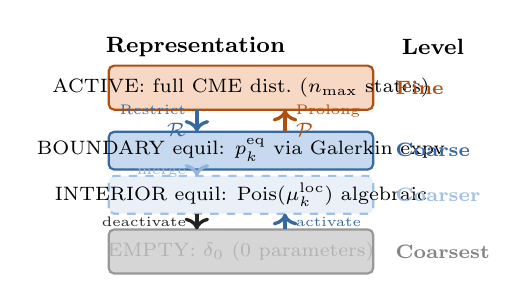
\begin{tikzpicture}[scale=0.80, every node/.style={font=\scriptsize}]
        % three "resolution levels" as horizontal bars
        \node[right,font=\footnotesize] at (-0.2,4.2) {\textbf{Representation}};
        \node[right,font=\footnotesize] at (4.5,4.2)  {\textbf{Level}};

        % fine
        \draw[fill=activecolor!25,draw=activecolor!80!black,thick,rounded corners=2pt]
          (0,3.2) rectangle (4.2,3.9);
        \node at (2.1,3.55) {ACTIVE: full CME dist.\ ($n_{\max}$ states)};
        \node[right] at (4.4,3.55) {\textcolor{activecolor!80!black}{\textbf{Fine}}};

        % medium-hi: boundary equil
        \draw[fill=equilcolor!30,draw=equilcolor!80!black,thick,rounded corners=2pt]
          (0,2.25) rectangle (4.2,2.85);
        \node at (2.1,2.56) {BOUNDARY equil: $p_k^{\rm eq}$ via Galerkin expv};
        \node[right] at (4.4,2.56) {\textcolor{equilcolor!80!black}{\textbf{Coarse}}};
        % medium-lo: interior equil
        \draw[fill=equilcolor!12,draw=equilcolor!50,thick,rounded corners=2pt,dashed]
          (0,1.55) rectangle (4.2,2.15);
        \node at (2.1,1.85) {INTERIOR equil: $\Pois(\mu_k^{\rm loc})$ algebraic};
        \node[right] at (4.4,1.85) {\textcolor{equilcolor!50}{\textbf{Coarser}}};

        % coarsest
        \draw[fill=emptycolor!20,draw=emptycolor!50,thick,rounded corners=2pt]
          (0,0.6) rectangle (4.2,1.3);
        \node[text=white!70!black] at (2.1,0.95) {EMPTY: $\delta_0$ (0 parameters)};
        \node[right] at (4.4,0.95) {\textcolor{emptycolor!60}{\textbf{Coarsest}}};

        % restrict arrows
        \draw[->,very thick,equilcolor!80!black]
          (1.4,3.2) -- (1.4,2.85)
          node[midway,left,align=right]{\tiny Restrict\\$\calR$};
        \draw[->,very thick,equilcolor!60]
          (1.4,2.25) -- (1.4,2.15)
          node[midway,left,align=right]{\tiny merge};
        \draw[->,very thick,emptycolor!70!black]
          (1.4,1.55) -- (1.4,1.3)
          node[midway,left,align=right]{\tiny deactivate};

        % prolong arrows
        \draw[->,very thick,activecolor!80!black]
          (2.8,2.85) -- (2.8,3.2)
          node[midway,right,align=left]{\tiny Prolong\\$\calP$};
        \draw[->,very thick,equilcolor!80!black]
          (2.8,1.3) -- (2.8,1.55)
          node[midway,right,align=left]{\tiny activate};
      \end{tikzpicture}
      \end{center}

      \vspace{0.2em}
      {\scriptsize
        Four levels: active / boundary-equil / interior-equil / empty.
        Galerkin coarse operator $A_c{=}\calR A\calP$ used for boundary equil;
        algebraic mean for interior (no matrix exp).
      }
    \end{column}
  \end{columns}

\end{frame}


% ================================================================
% 7. Algorithm summary
% ================================================================
\begin{frame}[shrink=4]{Algorithm: one time step}

\vspace{-0.1cm}
\begin{columns}[T]
  \begin{column}{0.54\textwidth}
    \begin{enumerate}\setlength\itemsep{0.28em}
      \item \textbf{Compute effective means.}\\
            Active: $\mu_k {=} \langle p_k \rangle$.
            Equil: $\mu_k {=} \langle p_k^{\rm eq} \rangle$ (from stored dist.).

      \item \textbf{Evolve active voxels} (full CME, Krylov $m$).\\
            $p_k \leftarrow e^{Q_k \Delta t} p_k$,\;
            $Q_k = Q(k_b {+} d\sum_{\ell} \mu_\ell,\; k_d {+} d|\text{nb}|)$.

      \item \textbf{Update equilibrated voxels} (Galerkin $A_c{=}\calR A\calP$).\\
            \textcolor{equilcolor!80!black}{\textit{Boundary}} ($\exists$ active nb):
            $p_k^{\rm eq} \leftarrow e^{Q_k^{\rm eq}\Delta t}p_k^{\rm eq}$,
            small Krylov $m_{\rm eq} \ll m$.\\
            \textcolor{equilcolor!50}{\textit{Interior}} (all nb equil/empty):
            $p_k^{\rm eq} \leftarrow \Pois(\mu_k^{\rm loc})$, algebraic.

      \item \textbf{Accumulate flux} into empty voxels from active+equil.\\
            $\Phi_k \mathrel{+}= d\,\mu_\ell\,\Delta t$.

      \item \textbf{Prolong (activate).}
            $\Phi_k \ge \varepsilon_{\rm exp} \Rightarrow p_k = \delta_0$.

      \item \textbf{Restrict (deactivate).}
            $|\mu_k {-} \mu_k^{\rm loc}|/\mu_k^{\rm loc} < \varepsilon_{\rm eq}$
            \textbf{and} $d_{\rm TV}(p_k,\Pois(\mu_k^{\rm loc})) < \varepsilon_{\rm TV}$:
            set $p_k^{\rm eq} \leftarrow p_k$ (no information lost).
    \end{enumerate}
  \end{column}
  \begin{column}{0.42\textwidth}
    \begin{block}{Cost per step (three tiers)}
      \vspace{0.1em}
      \begin{tabular}{@{}llc@{}}
        \toprule
        Tier & Count & Work \\
        \midrule
        Active & $K_{\rm act}$ & expv$(n_{\max},m)$ \\
        Boundary equil & $O(\sqrt{K})$ & expv$(n_{\rm eq},m_{\rm eq})$ \\
        Interior equil & $O(K_{\rm eq})$ & $O(n_{\rm eq})$ algebraic \\
        \bottomrule
      \end{tabular}\\[0.3em]
      {\scriptsize
        $K_{\rm act} \ll K$ (wavefront ring only).
        $m_{\rm eq} \ll m$ (near-Poisson $\Rightarrow$ fast Krylov).
        Interior equil: no matrix exp at all.
      }
    \end{block}

    \vspace{0.3em}
    \begin{block}{State-space comparison}
      \vspace{0.1em}
      \begin{tabular}{@{}lc@{}}
        \toprule
        Method & States tracked \\
        \midrule
        Full FSP & $n_{\max}^{SK}$ \\
        Spatial adaptive FSP & $K_{\rm act} \cdot n_{\max}^{S}$ \\
        \bottomrule
      \end{tabular}
    \end{block}
  \end{column}
\end{columns}

\end{frame}


% ================================================================
% 7b. Galerkin coarse operator — boundary vs interior
% ================================================================
\begin{frame}{Galerkin coarse operator: boundary vs.\ interior equilibrated voxels}

\begin{columns}[T]
  \begin{column}{0.50\textwidth}
    \textbf{The Galerkin coarse operator} for a single voxel $k$:\\[0.3em]
    Marginalise $A_{\rm RDME}$ over all other voxels assuming independence
    (mean-field $n_\ell \to \mu_\ell$):
    \[
      A_c^{(k)} = \underbrace{Q(k_b {+} d\textstyle\sum_\ell\mu_\ell,\; k_d {+} d|\text{nb}|)}_{
        \text{single-voxel birth-death CME with eff.\ rates}}.
    \]
    This is \emph{exactly} what \texttt{build\_coarse\_system} derives
    for one voxel of the coarsened RDME.

    \bigskip
    \textbf{Two update rules depending on neighbourhood:}

    \medskip
    \begin{tabular}{@{}p{0.42\textwidth}p{0.52\textwidth}@{}}
      \textcolor{equilcolor!80!black}{\textbf{Boundary}} &
      \textcolor{equilcolor!50!black}{\textbf{Interior}} \\[0.2em]
      $\ge 1$ active nb & all nb equil/empty \\[0.2em]
      $p_k^{\rm eq} \!\leftarrow e^{A_c^{(k)}\Delta t}p_k^{\rm eq}$ &
      $p_k^{\rm eq} \leftarrow \Pois(\mu_k^{\rm loc})$ \\[0.2em]
      Krylov $m_{\rm eq}{=}8$ & algebraic, $O(n_{\rm eq})$ \\[0.2em]
      Rates change fast & Rates change slowly \\[0.2em]
      Near wavefront & Deep interior \\
    \end{tabular}
  \end{column}
  \begin{column}{0.46\textwidth}
    \begin{center}
    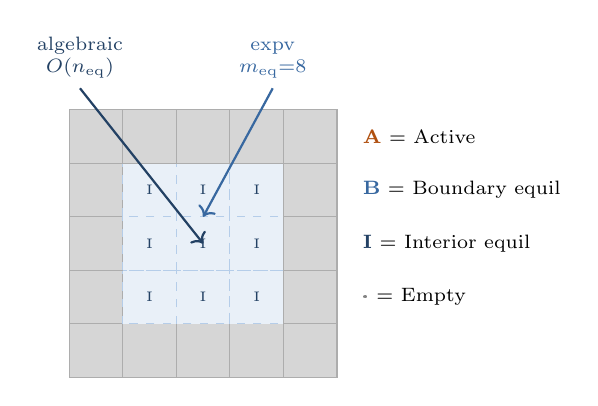
\begin{tikzpicture}[scale=0.68, every node/.style={font=\scriptsize}]
      % Grid snapshot: 5×5
      \def\G{5}
      % Colors: 0=empty, 1=active, 2=boundary-equil, 3=interior-equil
      % Pattern (approx): interior=3, boundary=2, active=1, empty=0
      % Row 5 (top): 0 0 0 0 0
      % Row 4:       0 0 2 0 0
      % Row 3:       0 2 1 2 0
      % Row 2:       0 2 3 2 0  -- wait let me think
      % Actually: interior equil = fully surrounded by equil/empty
      %           boundary equil = adjacent to active
      % Let active be at (3,3) i.e. center
      % boundary equil: (3,2),(3,4),(2,3),(4,3)
      % interior equil: (2,2),(2,4),(4,2),(4,4) -- not adjacent to active
      % Actually interior equil requires ALL neighbors equil/empty, so:
      % (2,2): neighbors are (1,2),(3,2),(2,1),(2,3) -- (3,2) is boundary equil...
      % So (2,2) IS adjacent to boundary equil which is equil, not active -> interior OK
      % Let me define a cleaner pattern:
      % Active: (3,3)
      % Boundary equil (adj to active): (2,3),(4,3),(3,2),(3,4)
      % Interior equil (not adj to active): (1,3),(5,3),(3,1),(3,5),(2,2),(2,4),(4,2),(4,4),(1,1),(1,2),(2,1)...
      % Empty: rest
      % Simplified for 5x5:

      \foreach \row in {1,...,\G} {
        \foreach \col in {1,...,\G} {
          % Determine state: 0=empty,1=active,2=bnd-equil,3=int-equil
          \pgfmathtruncatemacro{\state}{
            (\row==3 && \col==3) ? 1 :
            ((\row==2 && \col==3)||(\row==4 && \col==3)||(\row==3 && \col==2)||(\row==3 && \col==4)) ? 2 :
            ((\row>=2 && \row<=4) && (\col>=2 && \col<=4)) ? 3 :
            0
          }
          \ifnum\state=0
            \fill[emptycolor!20] (\col-1,\row-1) rectangle (\col,\row);
            \draw[emptycolor!40,thin] (\col-1,\row-1) rectangle (\col,\row);
          \fi
          \ifnum\state=1
            \fill[activecolor!40] (\col-1,\row-1) rectangle (\col,\row);
            \draw[activecolor!80!black,thick] (\col-1,\row-1) rectangle (\col,\row);
            \node[activecolor!80!black,font=\tiny\bfseries] at (\col-0.5,\row-0.5) {A};
          \fi
          \ifnum\state=2
            \fill[equilcolor!30] (\col-1,\row-1) rectangle (\col,\row);
            \draw[equilcolor!80!black,thick] (\col-1,\row-1) rectangle (\col,\row);
            \node[equilcolor!70!black,font=\tiny] at (\col-0.5,\row-0.5) {B};
          \fi
          \ifnum\state=3
            \fill[equilcolor!12] (\col-1,\row-1) rectangle (\col,\row);
            \draw[equilcolor!40,thin,dashed] (\col-1,\row-1) rectangle (\col,\row);
            \node[equilcolor!50!black,font=\tiny] at (\col-0.5,\row-0.5) {I};
          \fi
        }
      }

      % Legend
      \node[right] at (5.3,4.5) {\textcolor{activecolor!80!black}{\textbf{A}} = Active};
      \node[right] at (5.3,3.5) {\textcolor{equilcolor!80!black}{\textbf{B}} = Boundary equil};
      \node[right] at (5.3,2.5) {\textcolor{equilcolor!50!black}{\textbf{I}} = Interior equil};
      \node[right] at (5.3,1.5) {\textcolor{emptycolor!60}{\textbf{·}} = Empty};

      % Cost annotation
      \draw[<-,equilcolor!80!black,thick]  (2.5,3.0) -- (3.8,5.4)
        node[above,align=center,equilcolor!80!black]
          {expv\\$m_{\rm eq}{=}8$};
      \draw[<-,equilcolor!50!black,thick] (2.5,2.5) -- (0.2,5.4)
        node[above,align=center,equilcolor!50!black]
          {algebraic\\$O(n_{\rm eq})$};
    \end{tikzpicture}
    \end{center}

    \vspace{0.2em}
    {\scriptsize
      At any instant, \textbf{boundary equil} $=O(\sqrt{K})$ voxels
      (wavefront circumference).  Interior equil $=O(K)$ but costs
      only $O(n_{\rm eq})$ each --- no matrix exponential.
    }
  \end{column}
\end{columns}

\end{frame}


% ================================================================
% 8. Results: 2D birth-death wavefront
% ================================================================
\begin{frame}{2D birth-death: wavefront propagation and collapse}

  \begin{columns}[T]
    \begin{column}{0.52\textwidth}
      \textbf{Model.}\;
      $\emptyset \xrightarrow{k_b} A \xrightarrow{k_d} \emptyset$ in each voxel
      with diffusion $D$.
      Steady state: each voxel independent $\Pois(k_b/k_d)$.

      \medskip
      \textbf{IC.}\; All voxels empty; center voxel activated at $t=0$.
      Birth reactions seed the wavefront.

      \medskip
      \textbf{Parameters:}\;
      $K{=}14$, $k_b{=}1$, $k_d{=}0.5$, $D{=}1$, $\mu^*{=}2$.

      \bigskip
      \textbf{Voxel state counts over time:}
      \begin{itemize}\setlength\itemsep{0.3em}
        \item Active count peaks at $\sim$66 (one wavefront ring),
              \textbf{not} $K^2 = 196$.
        \item Equilibrated count grows monotonically behind the front.
        \item Active $\to 0$: the distribution is
              \emph{fully represented by coarse parameters}.
      \end{itemize}

      \medskip
      \textbf{ODE comparison.}\;
      Naive $K^2 k_b$ ODE \emph{over}estimates: empty voxels do not birth.
      Corrected ODE $(K^2 - K_{\rm empty})k_b - k_d \langle N\rangle$ matches FSP.
    \end{column}
    \begin{column}{0.44\textwidth}
      \begin{center}
      \includegraphics[width=\textwidth]{birthdeath_2d_spatial.png}
      \end{center}
    \end{column}
  \end{columns}

\end{frame}


% ================================================================
% 9. Results: center voxel dynamics
% ================================================================
\begin{frame}{Center voxel: two-phase equilibration}

  \begin{columns}[T]
    \begin{column}{0.54\textwidth}
      The center voxel is activated at $t = 0$ and deactivated
      \textbf{early} once its distribution reaches its \emph{local} SS.

      \medskip
      \textbf{Local SS} (4 empty neighbours):
      \[
        \mu^{\rm loc}_{\rm center}
        = \frac{k_b}{k_d + 4d}
        = \frac{1}{0.5 + 4}
        \approx 0.22.
      \]
      The center's stored mean then \textbf{evolves upward} as ring-1,
      ring-2, \ldots equilibrate behind the wavefront.

      \bigskip
      \textbf{Two phases of the center mean:}
      \begin{enumerate}\setlength\itemsep{0.4em}
        \item \textcolor{activecolor}{\textbf{Fast:}}
              $\mu \nearrow 0.22$ in $\sim 1/k_d^{\rm eff} \approx 0.2$ time units.
              Deactivated.
        \item \textcolor{equilcolor}{\textbf{Slow:}}
              $\mu^{\rm loc} \nearrow 2.0$ over $\tau_{\rm diff} \approx (K/2)^2/(2D) \approx 24$
              time units as successive rings equilibrate.
      \end{enumerate}

      \bigskip
      This \textbf{staircase} in $\mu^{\rm loc}$ traces the equilibration
      wave propagating inward from each newly-equilibrated ring.
    \end{column}
    \begin{column}{0.42\textwidth}
      \begin{center}
      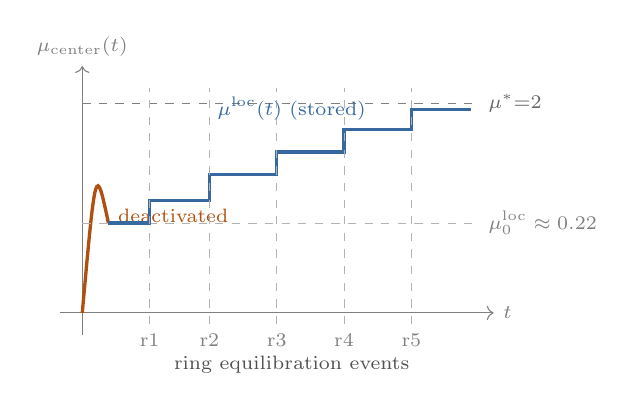
\begin{tikzpicture}[scale=0.95, every node/.style={font=\scriptsize}]
        \draw[->,black!50] (-0.3,0) -- (5.5,0) node[right]{$t$};
        \draw[->,black!50] (0,-0.3) -- (0,3.3) node[above]{$\mu_{\rm center}(t)$};

        % global SS line
        \draw[dashed,black!50,thin] (0,2.8) -- (5.3,2.8);
        \node[right,black!60] at (5.3,2.8) {$\mu^*{=}2$};

        % fast rise to local SS
        \draw[activecolor!80!black,very thick] (0,0) .. controls (0.18,2.0) .. (0.35,1.2);
        \node[activecolor!80!black,right] at (0.35,1.3) {deactivated};
        \draw[dashed,black!30] (0,1.2) -- (5.3,1.2);
        \node[right,black!50] at (5.3,1.2) {$\mu^{\rm loc}_0 \approx 0.22$};

        % staircase of stored mean updates
        \draw[equilcolor!80!black,very thick]
          (0.35,1.2) -- (0.9,1.2)
          -- (0.9,1.5)   % ring 1 equilibrates
          -- (1.7,1.5)
          -- (1.7,1.85)  % ring 2
          -- (2.6,1.85)
          -- (2.6,2.15)  % ring 3
          -- (3.5,2.15)
          -- (3.5,2.45)  % ring 4
          -- (4.4,2.45)
          -- (4.4,2.72)  % ring 5
          -- (5.2,2.72);

        % ring labels
        \foreach \x/\lbl in {0.9/r1, 1.7/r2, 2.6/r3, 3.5/r4, 4.4/r5} {
          \draw[black!30,thin,dashed] (\x,-0.15) -- (\x,3.0);
          \node[below,black!50] at (\x,-0.15) {\lbl};
        }
        \node[above,equilcolor!80!black] at (2.8,2.45) {$\mu^{\rm loc}(t)$ (stored)};
        \node[below,mygray] at (2.8,-0.45) {ring equilibration events};
      \end{tikzpicture}
      \end{center}
    \end{column}
  \end{columns}

\end{frame}


% ================================================================
% 10. Collapse to single CME
% ================================================================
\begin{frame}[shrink=5]{Collapse to a single well-mixed CME}

  \begin{columns}[T]
    \begin{column}{0.52\textwidth}
      Once all voxels are equilibrated:
      \begin{itemize}\setlength\itemsep{0.4em}
        \item All $\mu_k^{\rm loc} \to \mu^* = k_b/k_d = 2$.
        \item No active voxels remain; FSP support = $\emptyset$.
        \item Total count $N = \sum_k n_k$ is independent of
              spatial arrangement.
      \end{itemize}

      \medskip
      The \textbf{collapsed CME} for $N$ is:
      \[
        \emptyset \;\xrightarrow{K^2 k_b}\; N \;\xrightarrow{k_d}\; \emptyset,
      \]
      with SS distribution $N^* \sim \Pois(K^2\mu^*)$.

      \bigskip
      \begin{block}{Product-form exactness}
        For birth-death, the voxels are independent at SS:
        $p^* = \prod_k \Pois(\mu^*)$.
        Total distribution is convolution of $K^2$ independent Poissons:
        \[
          N^* = \sum_{k=1}^{K^2} n_k^* \sim \Pois\!\bigl(K^2\mu^*\bigr).
        \]
        The FSP product-form distribution agrees with this \textbf{exactly}.
      \end{block}
    \end{column}
    \begin{column}{0.44\textwidth}
      \begin{center}
      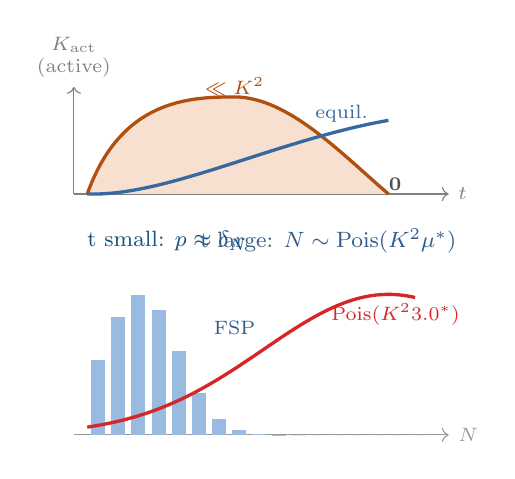
\begin{tikzpicture}[scale=0.85, every node/.style={font=\scriptsize}]
        % Timeline of active count
        \draw[->,black!50] (-0.2,3.6) -- (5.4,3.6) node[right]{$t$};
        \draw[->,black!50] (-0.2,3.6) -- (-0.2,5.2)
          node[above,align=center]{$K_{\rm act}$\\(active)};

        % arc: rises to peak, falls to 0
        \fill[activecolor!20]
          (0,3.6) .. controls (0.5,5.0) and (1.5,5.05) .. (2.2,5.05)
          .. controls (3.0,5.05) and (3.8,4.2) .. (4.5,3.6) -- (0,3.6);
        \draw[activecolor!80!black,very thick]
          (0,3.6) .. controls (0.5,5.0) and (1.5,5.05) .. (2.2,5.05)
          .. controls (3.0,5.05) and (3.8,4.2) .. (4.5,3.6);
        \node[activecolor!80!black] at (2.2,5.2) {$\ll K^2$};

        \draw[equilcolor!80!black,very thick]
          (0,3.6) .. controls (1.2,3.56) and (2.8,4.4) .. (4.5,4.7);
        \node[equilcolor!80!black] at (3.8,4.8) {equil.};
        \node[mygray] at (4.6,3.75) {\textbf{0}};

        % Distribution panels
        \node[font=\footnotesize,myblue!70!black] at (1.2,2.9)
          {t small: $p \approx \delta_N$};
        \node[font=\footnotesize,equilcolor!70!black] at (3.6,2.9)
          {t large: $N \sim \Pois(K^2\mu^*)$};

        % Final total distribution sketch
        \draw[->,black!40] (-0.2,0) -- (5.4,0) node[right]{$N$};
        \pgfmathsetmacro{\mu}{3.0}
        \pgfmathsetmacro{\sig}{1.0}
        \foreach \x in {0,...,16} {
          \pgfmathsetmacro{\h}{exp(-(\x-\mu*3.5/5)*(\x-\mu*3.5/5)/(2*\sig*\sig*3.5))}
          \fill[equilcolor!55]
            ({\x*0.30+0.06},0) rectangle ({\x*0.30+0.27},\h*2.1);
        }
        \draw[slowred,very thick,domain=0:4.9,samples=80]
          plot (\x, {2.1*exp(-(\x-1.5*\mu)*(\x-1.5*\mu)/(2*\sig*\sig*3.5))});
        \node[slowred,right] at (3.5,1.8) {$\Pois(K^2\mu^*)$};
        \node[equilcolor!70!black] at (2.2,1.6) {FSP};
      \end{tikzpicture}
      \end{center}
    \end{column}
  \end{columns}

\end{frame}


% ================================================================
% 11. Summary and outlook
% ================================================================
\begin{frame}{Summary and outlook}

  \begin{columns}[T]
    \begin{column}{0.54\textwidth}
      \textbf{What we built:}
      \begin{itemize}\setlength\itemsep{0.45em}
        \item A spatially adaptive FSP for the RDME that maintains only a
              \textbf{sparse active set} — the current wavefront ring.
        \item Three-level representation: empty ($\delta_0$),
              equilibrated ($\Pois(\mu^{\rm loc})$), active (full CME).
        \item Physics-driven prolong/restrict cycle:
              \textbf{an adaptive multigrid V-cycle in state space}.
      \end{itemize}

      \bigskip
      \textbf{Key properties:}
      \begin{itemize}\setlength\itemsep{0.35em}
        \item Computational work $\propto K_{\rm act} \cdot n_{\max}$,
              \textbf{not} $n_{\max}^K$.
        \item Mean-field coupling is exact at SS for linear kinetics.
        \item Equilibrated means evolve algebraically (local SS tracking).
        \item Total distribution collapses to $\Pois(K^2\mu^*)$.
      \end{itemize}
    \end{column}
    \begin{column}{0.42\textwidth}
      \textbf{Open directions:}
      \begin{enumerate}\setlength\itemsep{0.45em}
        \item \textbf{Nonlinear kinetics} (Schlögl, bistable networks).\\
              Mean-field is no longer exact. Need joint tracking at
              wavefront pairs (patch QSD).
        \item \textbf{Joint wavefront tracking.}\\
              When $K_{\rm act}$ voxels are correlated, maintain a
              \emph{joint} distribution rather than independent marginals.
        \item \textbf{Adaptive re-activation.}\\
              Re-activate equilibrated voxels when perturbations arrive
              (e.g., front reflections, new injections).
        \item \textbf{Higher dimensions and irregular grids.}\\
              The prolong/restrict logic generalises to 3-D and
              unstructured meshes.
      \end{enumerate}
    \end{column}
  \end{columns}

\end{frame}


\end{document}
